\chapter{Exhaustive PRN search}
  \section{Previous work}

  As shown in the previous chapter, arithmetic methods for finding sequences
  with a low off-peak autocorrelation have huge constraints on the length of
  the generated sequences. To overcome this limitation, exhaustive searches
  through the possible permutations have been conducted in the past. This
  exhaustive searchs have, if not properly optimized, a search space of
  $O(2^n)$, where $n$ is the length of the binary sequence, which make their
  results very limited in size compared to the arithmetic methods.\\

  One of the first optimizations for this method was
  proposed by \citet{Mertens_1996} in which he provided an algorythm
  with a complexity of $O(1.85^n)$. In his work, he applied a branch and bound
  algorythm that rules out the equivalent sequences and sets a minimum bound
  to the autocorrelation based on how complementing a single symbol of the
  sequence affects the autocorrelation.\\

  \begin{itemize}
    \item Records y como se consiguieron
    \item Complejidad de los métodos
  \end{itemize}
  \section{Our approach}

  To tackle the huge complexity encountered in the previous methods, we took
  a different approach. Instead of dealing with the combinatorial explosion
  of all the possible binary sequences of length $N$, we decided to work with
  a smaller set consisting on all the possible sequences which can be
  constructed through the composition method with Legendre base sequences.\\

  This approach haves some pros and cons:

  \begin{itemize}
    \item The search space for sequences of length $N$ is reduced from $O(2^N)$
          to $O(p^m)$ where $p*m = N$.
    \item The autocorrelation function can be optimized for the composition
          method (as we will see in a following chapter).
    \item The search space can be efficiently bounded applying the Hamming
          autocorrelation.
    \item Unfortunatly, the possible sequences that we can find by this method
          are limited in length. We can only get sequences of the form $p * m$
          where $p$ is prime and $gcd(p, m) = 1$.
  \end{itemize}

  Given a base sequence of size $n$ and a length $m$ for the shift sequences,
  our program needs to find all the shift sequences that generate a composite
  sequence with a good autocorrelation.\\

  This means that the search space are all the posible permutations of the
  shift sequence, in other words, $n^m$ permutations. However, there are some
  relations between the different shift sequences that let us narrow the
  search space.\\

  For example, if we add a constant to every component to the shift sequence,
  we get a shifted version of the same sequence. This means that if we only
  computed the permutations that start with the same component, we would cover
  the whole search space as any other permutations would just be shifts of
  one permutation from the computed set. This optimization narrows our
  search space to $n^{(m-1)}$.\\

  Other optimization arises from the form of the shift sequences. In general,
  if the symbols are repeated often, they trend to generate higher
  autocorrelation spikes or periods inside the composite sequence. This
  concept can be easily expressed with the Hamming autocorrelation function:\\

  \begin{definition}[Hamming autocorrelation]
    Given a sequence $S$ of length $n$ and the function $shift$ defined at
    Equation \ref{eq:3}, we define the Hamming autocorrelation as:
      \begin{equation}
        HA(S)_{\tau} = \sum_{i=0}^{n} HAComponent(S_{\tau}, shift(S, \tau)_{\tau})
      \end{equation}
    where $HAComponent$ is defined as:
      \begin{equation}
        HAComponent(c1, c2) = \left\{\begin{array}{lr}
            1  &  c1 = c2\\
            0  & \textnormal{otherwise} \\
        \end{array}\right.
      \end{equation}
  \end{definition}

  For our branch and bound algorythm, it's important to note that if we
  substitute a symbol that only appears once for another, the hamming
  autocorrelation won't get lower. This means that if we do a depth-in-first
  bounding the nodes that have a hamming autocorrelation higher than the
  threshold (we mean, the maximum non trivial component), we are sure that all
  nodes in that branch have a higher hamming autocorrelation than the
  threshold.\\

  \begin{figure}[ht!]
    \begin{center}
      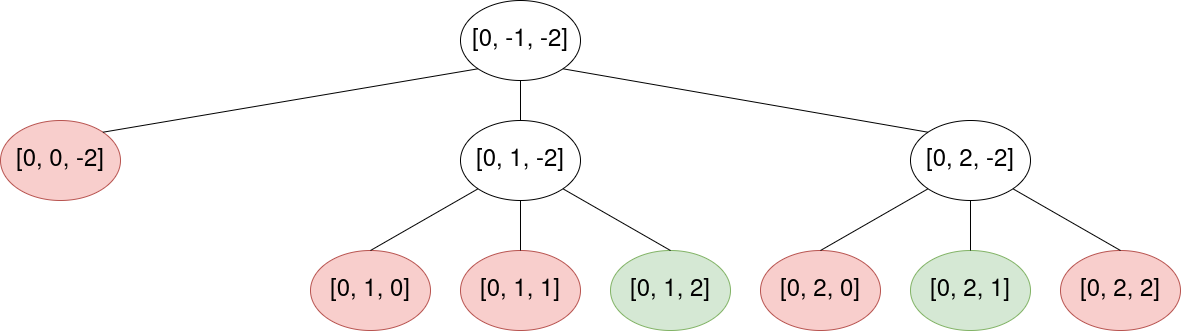
\includegraphics[scale=0.4]{Chapters/Implementation/Example_branch_bound.png}
    \end{center}
    \caption{An example of the branch and bound algorythm with a threshold for
    hamming autocorrelation of 1 and a base sequence of length 3. Red nodes
    represent prunes and green ones final nodes in which the
    autocorrelation is computed and checked. Negative values represent those
    that haven't been initialized yet.}
    \label{bb:fig:1}
  \end{figure}

  We can deduce several things from Figure \ref{bb:fig:1}:
  \begin{itemize}
    \item We reduce the number of autocorrelations computed by a significant
    amount.
    \item The computation on each branch isn't balanced. This must be taken
    into account when we design the parallelism model.
  \end{itemize}

  Como hemos reducido el espacio de búsqueda

  Las limitaciones en longitud(producto de 2 primos diferentes)

  Tabla de resultados

  Valor máximo esperado de la autocorrelación de una secuencia aleatoria
